\chapter{Проектирование и программная реализация прототипа веб-сервиса}
\label{chapter3}

\begin{annotation}
      В данной главе описывается процесс проектирования и программной реализации прототипа веб-сервиса с естественно-языковым интерфейсом. На основе сформулированных в предыдущей главе требований, с использованием языка моделирования UML, разрабатывается архитектура системы. Представляются диаграммы вариантов использования, компонентов и последовательности, которые детально описывают как статическую структуру, так и динамику взаимодействия элементов системы. В завершение приводится описание выбранного технологического стека и ключевых аспектов реализации прототипа.
\end{annotation}

\section{Проектирование архитектуры системы с использованием UML}

Проектирование является критически важным этапом разработки любого программного продукта. Для визуализации и формализации архитектуры будущего веб-сервиса был использован унифицированный язык моделирования UML (Unified Modeling Language). Были построены три диаграммы, описывающие систему с разных уровней абстракции.

\subsection{Диаграмма вариантов использования (Use Case Diagram)}

Диаграмма вариантов использования является наиболее высокоуровневым представлением системы. Она определяет границы системы, ее основных действующих лиц (акторов) и цели, которые эти акторы могут достигать при взаимодействии с системой.

Для нашего веб-сервиса был определен один актор~--- \textbf{Пользователь}. Его основные цели (варианты использования) представлены на рис.~\ref{fig:use-case-diagram}.

\begin{figure}[ht]
      \centering
      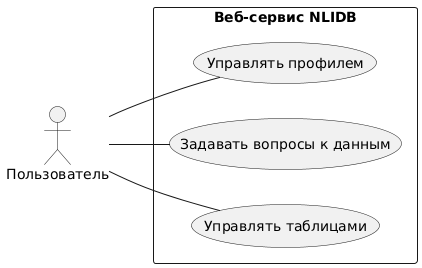
\includegraphics[width=0.7\textwidth]{created-diagrams/uml/use-case-diagram.png}
      \caption{Диаграмма вариантов использования}
      \label{fig:use-case-diagram}
\end{figure}

Как видно из схемы, Пользователь может выполнять три ключевые функции:
\begin{compactitem}
      \item \textbf{Управлять таблицами}. Этот вариант использования включает в себя загрузку
      новых таблиц (CSV/Excel), их переименование и удаление, а также добавление
      описаний для столбцов.
      \item \textbf{Задавать вопросы к данным}. Основная функция системы,
      позволяющая пользователю формулировать запросы на естественном языке к выбранной таблице.
      \item \textbf{Управлять профилем}. Включает в себя регистрацию, аутентификацию и
      изменение данных своего аккаунта (псевдоним, пароль, аватар).
\end{compactitem}

\subsection{Диаграмма компонентов (Component Diagram)}

Диаграмма компонентов описывает физическую структуру системы, показывая,
из каких крупных программных блоков она состоит и как они связаны между собой.
Эта диаграмма является основной архитектурной схемой нашего веб-сервиса
(см.~рис.~\ref{fig:component-diagram}).

\begin{figure}[ht]
      \centering
      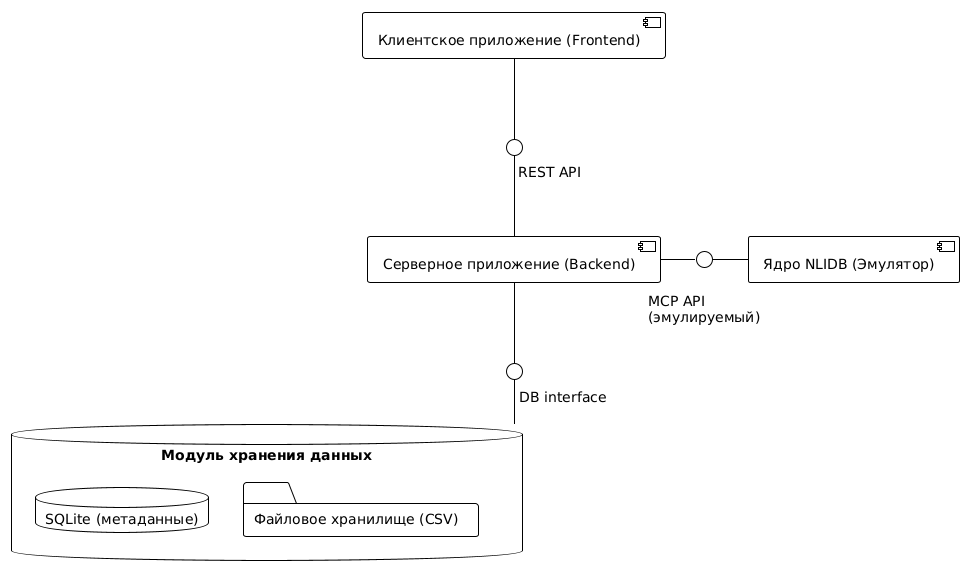
\includegraphics[width=1\textwidth]{created-diagrams/uml/component-diagram.png}
      \caption{Диаграмма компонентов системы}
      \label{fig:component-diagram}
\end{figure}

Система состоит из четырех основных компонентов:
\begin{compactenum}
      \item \textbf{Клиентское приложение (Frontend):} Компонент, работающий в браузере пользователя.
      Реализован на HTML/CSS/JS. Отвечает за пользовательский интерфейс и взаимодействие с
      бэкендом через REST API.
      \item \textbf{Серверное приложение (Backend):} Основной компонент, реализованный на
      Python с использованием фреймворка FastAPI. Он предоставляет REST API,
      управляет бизнес-логикой и выступает в роли организатора для других компонентов.
      \item \textbf{Модуль хранения данных:} Отвечает за персистентное хранение информации.
      Он состоит из базы данных \textbf{SQLite} для метаинформации
      (пользователи, таблицы, описания столбцов) и \textbf{Файлового хранилища} для
      загруженных CSV/Excel файлов и аватаров пользователей.
      \item \textbf{Ядро NLIDB (Эмулятор):} В рамках прототипа~--- это компонент-эмулятор,
      имитирующий работу настоящего XiYan-SQL MCP Server. Он предоставляет внутренний API,
      который полностью соответствует спроектированному протоколу взаимодействия с целевой системой.
\end{compactenum}

\subsection{Диаграмма последовательности (Sequence Diagram)}

Диаграмма последовательности детализирует взаимодействие между компонентами во времени.
Она наглядно демонстрирует, какие вызовы и в какой последовательности происходят для
выполнения конкретного варианта использования. На рис.~\ref{fig:sequence-diagram} показана
последовательность действий для самого важного сценария~--- обработки запроса пользователя на
естественном языке.

\begin{figure}[ht]
      \centering
      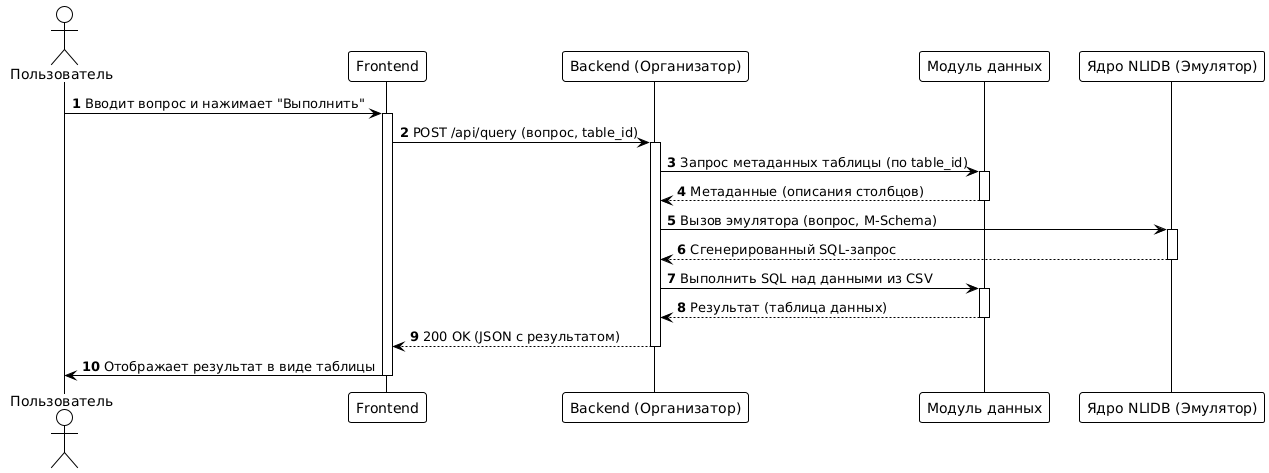
\includegraphics[width=\textwidth]{created-diagrams/uml/sequence-diagram.png}
      \caption{Диаграмма последовательности для обработки ЕЯ-запроса}
      \label{fig:sequence-diagram}
\end{figure}

Процесс, изображенный на диаграмме, состоит из следующих шагов:
\begin{compactenum}
      \item Пользователь вводит вопрос в интерфейсе и нажимает кнопку <<Выполнить>>.
      \item \textbf{Frontend} отправляет асинхронный \verb|POST| запрос на эндпоинт
      \verb|/api/query| \textbf{Backend}-сервера, передавая текст вопроса и ID выбранной таблицы.
      \item \textbf{Backend (Организатор)} получает запрос и\
      сначала обращается к \textbf{Модулю данных}, чтобы получить метаинформацию о таблице
      (путь к файлу, описания столбцов) из базы SQLite.
      \item Получив метаданные, \textbf{Backend} формирует из них M-Schema и
      обращается к \textbf{Ядру NLIDB (Эмулятору)}, передавая ему вопрос и схему.
      \item \textbf{Эмулятор} для тестовых сценариев возвращает заранее заготовленный SQL-запрос.
      \item \textbf{Backend} получает SQL. Он снова обращается к \textbf{Модулю данных},
      но на этот раз для выполнения операции: он считывает нужный CSV-файл в объект pandas
      DataFrame и выполняет над ним полученный SQL-запрос с помощью библиотеки \texttt{pandasql}.
      \item \textbf{Модуль данных} возвращает результат выполнения~--- новый DataFrame.
      \item \textbf{Backend} сериализует результирующий DataFrame в формат JSON и
      отправляет его обратно на \textbf{Frontend} в теле успешного HTTP-ответа.
      \item \textbf{Frontend} получает данные и отрисовывает их в виде таблицы для
      Пользователя.
\end{compactenum}

Данные диаграммы полностью описывают спроектированную архитектуру и
служат основой для этапа программной реализации.




\section{Выбор стека технологий}

На основе спроектированной в предыдущем разделе архитектуры был выбран конкретный стек
технологий для программной реализации прототипа. Выбор каждого инструмента и фреймворка
обусловлен функциональными требованиями проекта, необходимостью разработки прототипа и
возможностями для дальнейшего масштабирования системы.

\paragraph{Серверная часть (Backend)}. Для реализации серверной части был выбран язык
программирования \textbf{Python} и асинхронный веб-фреймворк \textbf{FastAPI}.
Этот выбор обусловлен следующими причинами:
\begin{compactitem}
      \item \textbf{Экосистема Python для ИИ и анализа данных}. Ключевое ядро системы,
      XiYan-SQL, написано на Python. Использование Python для бэкенда является наиболее
      нативным и эффективным решением, так как позволяет избежать сложностей межъязыкового
      взаимодействия и напрямую интегрировать необходимые библиотеки.
      \item \textbf{Высокая производительность FastAPI}. FastAPI построен на базе Starlette и Pydantic,
      что обеспечивает ему производительность, сопоставимую с решениями на Go и Node.js.
      Его асинхронная природа идеально подходит для обработки запросов, связанных с
      длительными операциями, такими как обращение к LLM.
      \item \textbf{Автоматическая документация API}. FastAPI автоматически генерирует
      интерактивную документацию для API (Swagger UI и ReDoc), что значительно упрощает
      процесс разработки, тестирования и отладки взаимодействия между клиентской и серверной частями.
      \item \textbf{Работа с данными}. Для манипуляции данными из загружаемых
      CSV-файлов используется библиотека \textbf{pandas}~--- де-факто стандарт для
      анализа данных в Python. Для выполнения SQL-запросов над объектами DataFrame
      используется библиотека \textbf{pandasql}, что позволяет обрабатывать данные из файлов так,
      как если бы они находились в реляционной базе данных.
\end{compactitem}

\paragraph{Клиентская часть (Frontend)}.
Для реализации пользовательского интерфейса был выбран базовый стек из
\textbf{HTML5, CSS3 и нативного JavaScript (Vanilla JS)} по следующим причинам:
\begin{compactitem}
      \item \textbf{Фокус на основной задаче}. Основная сложность и новизна проекта лежат в
      серверной части и архитектуре взаимодействия с NLIDB-ядром. Использование стандартного
      стека без тяжелых фреймворков (таких как React или Vue) позволяет сконцентрировать усилия
      на реализации ключевой функциональности.
      \item \textbf{Отсутствие зависимостей и простота развертывания}. Данный подход не требует
      сложной системы сборки и зависимостей (Node.js, npm), что упрощает разработку и
      развертывание прототипа.
      \item \textbf{Гибкость}. Спроектированный REST API полностью отделяет логику бэкенда от
      представления. Это означает, что в будущем клиентская часть может быть легко заменена на
      более современный фреймворк без каких-либо изменений в серверной архитектуре.
\end{compactitem}

\paragraph{База данных (Database)}.
Для хранения метаинформации (данные пользователей, сведения о загруженных таблицах и
описания столбцов) была выбрана легковесная встраиваемая СУБД \textbf{SQLite}. Вот причины, по
которым была выбрана именно она:
\begin{compactitem}
      \item \textbf{Серверная независимость}. SQLite не требует отдельного серверного процесса.
      База данных представляет собой один файл, что идеально подходит для прототипа и упрощает
      его переносимость и настройку.
      \item \textbf{Нативная поддержка в Python}. SQLite встроена в стандартную библиотеку Python,
      что избавляет от необходимости устанавливать внешние драйверы. Для удобной работы с базой
      данных используется \textbf{SQLAlchemy}~--- популярный ORM (Object-Relational Mapper),
      который позволяет работать с таблицами как с Python-объектами.
\end{compactitem}

Таким образом, выбранный технологический стек представляет собой сбалансированное решение,
которое позволяет быстро и эффективно реализовать прототип, полностью соответствующий
поставленным задачам, и при этом закладывает прочный фундамент для будущего развития и
усложнения системы.




\section{Описание программной реализации прототипа веб-сервиса}

На основе спроектированной архитектуры и выбранного стека технологий был реализован
программный прототип веб-сервиса. В данном разделе приводится описание ключевых модулей и
функций системы. Фрагменты исходного кода, иллюстрирующие реализацию, вынесены в приложение
(см.~прил.~\ref{appendix-B}).




\subsection{Описание реализованных функций и модулей}

Программный код проекта организован в модульную структуру, соответствующую современным
практикам разработки на FastAPI. Корневая директория содержит главный файл приложения
\verb|main.py|, файлы конфигурации и директории с различными компонентами системы:
\verb|api|, \verb|core|, \verb|db|, \verb|features|, \verb|services|.

\paragraph{Точка входа и конфигурация приложения}. Файл \verb|main.py| является точкой
входа в приложение. В нем создается экземпляр класса \verb|FastAPI|, настраиваются
middleware-компоненты (включая \verb|CORSMiddleware| для обработки кросс-доменных запросов),
монтируются директории для статических файлов (\verb|/static|) и загрузок (\verb|/uploads|),
а также подключаются все API-маршруты из модуля \verb|api|. Важной частью является функция
с жизненным циклом (\verb|lifespan|), которая при старте сервера создает необходимые директории,
например, для аватаров пользователей.

\paragraph{Модуль аутентификации и управления пользователями}.
Данная функциональность реализована в директории \verb|features/users/|.
\begin{compactenum}
      \item \textbf{Модель данных (\texttt{models.py})}. Описана модель \verb|User| с
      использованием SQLAlchemy ORM. Она содержит поля для хранения псевдонима,
      хэшированного пароля, URL аватара и флагов статуса пользователя (активен,
      суперпользователь, стандартный аватар).
      \item \textbf{Операции с данными (\texttt{crud.py})}. Реализован класс \verb|CRUDUser|,
      который инкапсулирует всю логику прямого взаимодействия с базой данных:
      создание пользователя, поиск по имени, аутентификация, обновление. Для хэширования
      паролей используется библиотека \verb|passlib| с алгоритмом bcrypt, что обеспечивает
      безопасное хранение учетных данных.
      \item \textbf{API эндпоинты (\texttt{api.py})}. Определены все публичные маршруты для
      работы с пользователями:
      \begin{compactenum}
            \item \verb|/register|: Регистрация нового пользователя с валидацией длины и
            формата псевдонима и пароля.
            \item \verb|/login/access-token|: Аутентификация пользователя и
            выдача JWT-токена доступа, который используется для авторизации всех
            последующих запросов.
            \item \verb|/me|, \verb|/me/username|, \verb|/me/password|: Маршруты для получения и
            обновления данных текущего пользователя.
            \item \verb|/me/avatar|: Эндпоинты для загрузки и удаления пользовательского аватара.
      \end{compactenum}
      \item \textbf{Сервис генерации аватаров (\texttt{services/avatar\_service.py})}. Выделенный
      сервис, который при регистрации или удалении кастомного аватара генерирует стандартное
      изображение с первой буквой псевдонима пользователя на цветном фоне, созданном на
      основе хэша от имени. Для генерации используется библиотека \verb|Pillow|.
\end{compactenum}

\paragraph{Модуль управления таблицами данных}.
Аналогично пользователям, логика работы с таблицами вынесена в модуль \verb|features/tables/|.
\begin{compactenum}
      \item \textbf{Модель данных (\texttt{models.py})}. Описана модель \verb|Table|,
      связанная с моделью \verb|User| отношением <<один-ко-многим>>. Хранит имя таблицы,
      оригинальное имя файла, путь к файлу на сервере и ID владельца.
      \item \textbf{Сервис обработки таблиц (\texttt{services/table\_service.py})}. Этот
      сервисный слой содержит основную бизнес-логику. Функция \verb|process_and_save_table|
      отвечает за получение загруженного файла, его валидацию
      (проверка расширения на \verb|.csv| или \verb|.xlsx|), очистку имени, проверку на
      дубликаты, сохранение файла на диск с уникальным именем (с помощью \verb|uuid|) и,
      наконец, вызов CRUD-функции для создания записи в БД. Функция \verb|get_table_preview|
      использует библиотеку \verb|pandas| для чтения файла и возвращает первые 5 строк,
      названия столбцов и общее количество строк.
      \item \textbf{API эндпоинты (\texttt{api.py})}. Предоставляют интерфейс для фронтенда:
      загрузка файла (\verb|/upload|), получение списка таблиц пользователя (\verb|/|) и
      удаление таблицы (\verb|/{table_id}|). Все маршруты защищены и требуют наличия токена
      аутентификации.
\end{compactenum}

\paragraph{Модуль обработки NL-запросов (Организатор и Эмулятор)}.
Это центральный модуль, реализующий основную функцию системы. В текущем прототипе он
состоит из двух частей:
\begin{compactenum}
      \item \textbf{Организатор:} Его роль выполняет обработчик эндпоинта
      \verb|/api/query/|. Он получает от клиента текст вопроса и ID таблицы,
      извлекает из БД метаданные, формирует из них M-Schema и передает их в ядро NLIDB.
      \item \textbf{Ядро NLIDB (Эмулятор):} Реализовано в виде функции-заглушки
      \verb|convert_text_to_sql| в файле \verb|services/text_to_sql_service.py|.
      Эта функция имитирует работу настоящего ядра XiYan-SQL. Для демонстрационных целей в
      ней реализована простая логика, которая возвращает заранее заготовленные SQL-запросы
      для нескольких ключевых слов.
\end{compactenum}

Пример реализации эмулятора приведен в листинге~\ref{lst:nli-core-mock}. Такая архитектура
с эмуляцией позволяет полностью протестировать сквозное взаимодействие всех компонентов системы,
отложив сложную интеграцию с реальным MCP-сервером на следующие этапы разработки.

После получения SQL-запроса от эмулятора, Организатор использует библиотеку \verb|pandasql|
для его выполнения над DataFrame, полученным из пользовательского CSV-файла, и
возвращает результат на клиентскую часть.




\subsection{Описание графического пользовательского интерфейса}

Графический пользовательский интерфейс (GUI) является ключевой точкой взаимодействия пользователя с
системой. При его проектировании основной упор был сделан на минимализм, интуитивность и простоту,
чтобы пользователи без технической подготовки могли легко освоить все функции сервиса. Интерфейс
полностью русифицирован.


\paragraph{Аутентификация пользователя}. Первое, с чем сталкивается пользователь, — это система
аутентификации. Она состоит из двух экранов: регистрации и входа.

На экране регистрации пользователю предлагается ввести псевдоним и пароль. Система предоставляет
немедленную обратную связь: проверяет, не занят ли псевдоним, и отображает требования к сложности
пароля, подсвечивая выполненные и невыполненные условия(см.~рис.~\ref{fig:registration}). Это помогает
пользователю с первого раза создать корректные учетные данные.

После успешной регистрации пользователь попадает на экран входа, где для доступа к системе достаточно
ввести свой псевдоним и пароль. В случае неверного ввода данных система отображает понятное сообщение
об ошибке(см.~рис.~\ref{fig:login}).

\begin{figure}[ht]
      \centering
      \begin{subfigure}[b]{0.48\textwidth}
            \centering
            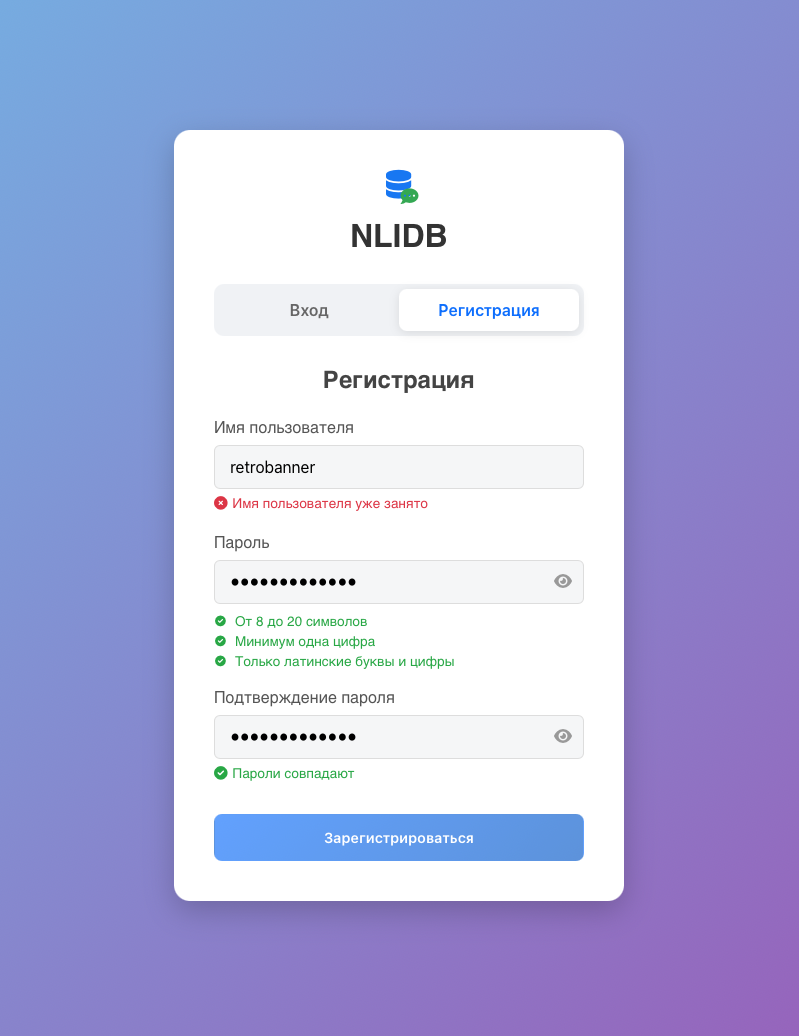
\includegraphics[width=\linewidth]{GUI/registration.png}
            \caption{Экран регистрации}
            \label{fig:registration}
      \end{subfigure}
      \hfill
      \begin{subfigure}[b]{0.48\textwidth}
            \centering
            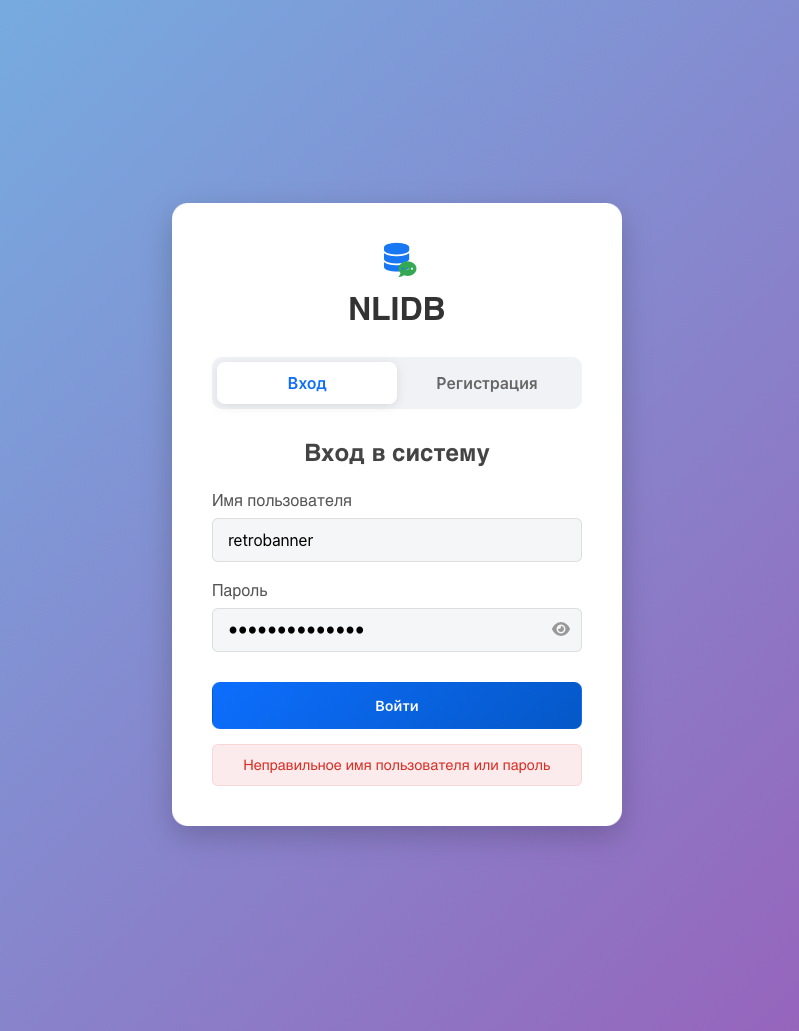
\includegraphics[width=\linewidth]{GUI/login.png}
            \caption{Экран входа в систему}
            \label{fig:login}
      \end{subfigure}
      \caption{Снимки экрана интерфейса аутентификации пользователя}
      \label{fig:auth_screens}
\end{figure}


\paragraph{Основной рабочий интерфейс}. После входа пользователь попадает на главный экран~---
«Конструктор запросов» (см.~рис.~\ref{fig:queries}). Это центральная рабочая область, разделенная на
две части. Слева расположена панель «Мои таблицы», где отображается список всех загруженных
пользователем таблиц. Кнопка «+» позволяет инициировать процесс добавления новой таблицы.

\begin{figure}[ht]
      \centering
      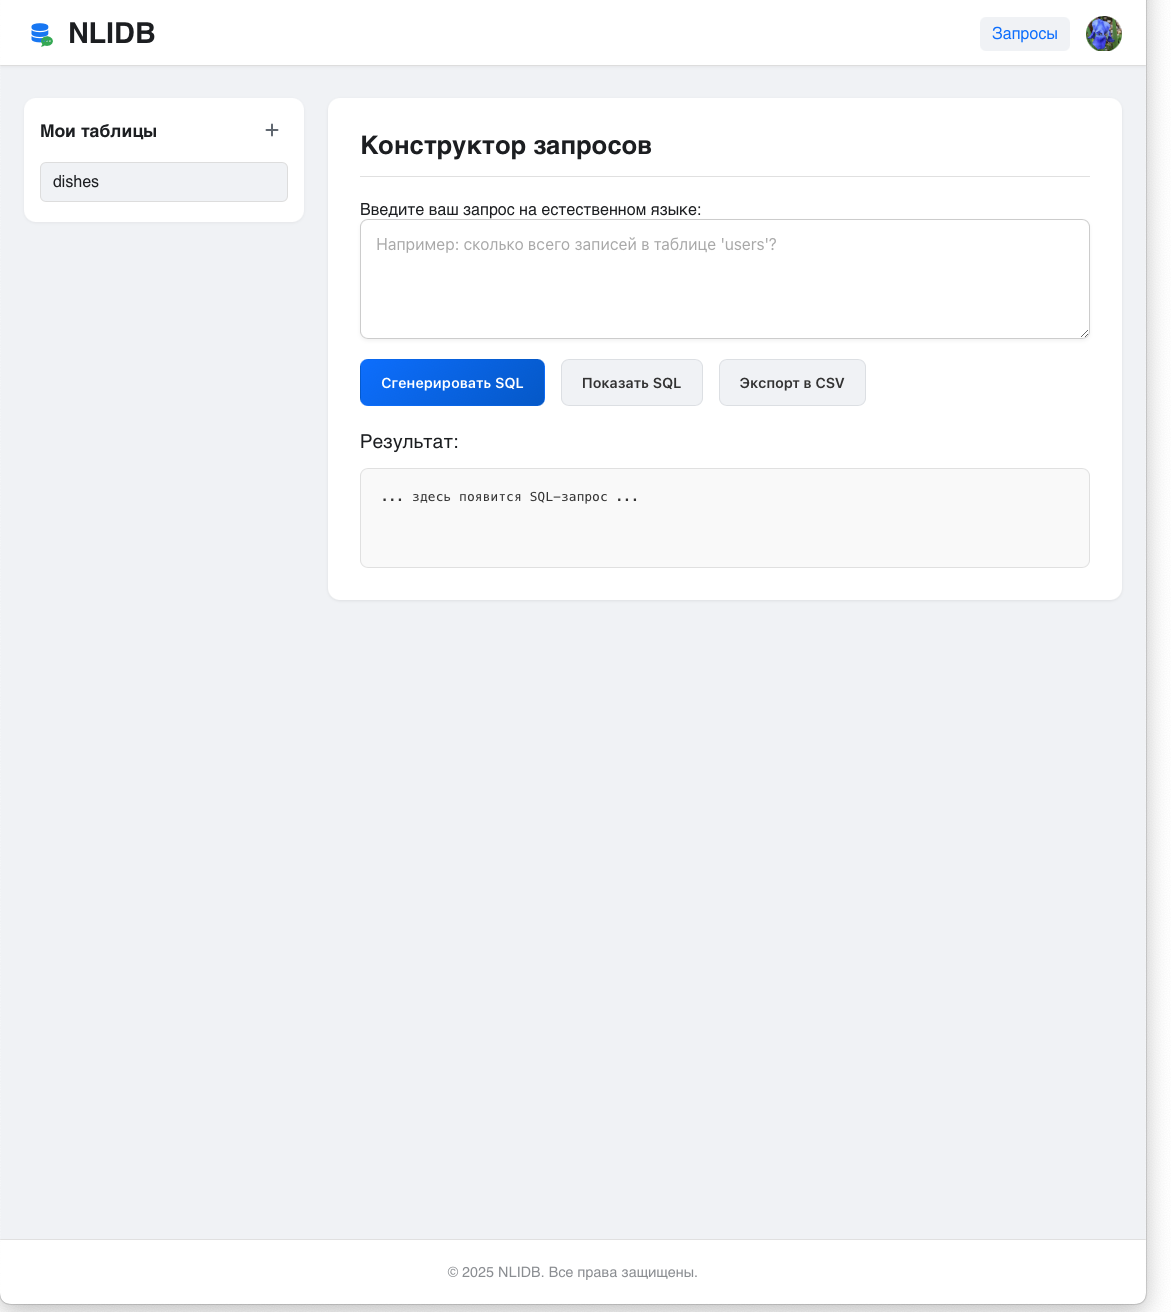
\includegraphics[width=\textwidth]{GUI/queries.png}
      \caption{Основной интерфейс конструктора запросов}
      \label{fig:queries}
\end{figure}

При нажатии на кнопку добавления таблицы открывается модальное окно
(см.~рис.~\ref{fig:table-uploading}), через которое пользователь может загрузить файл в формате CSV
или Excel. После выбора файла система автоматически анализирует его и отображает предварительный
просмотр первых 10 строк, что позволяет пользователю убедиться в корректности данных перед их
окончательной загрузкой.

\begin{figure}[ht]
      \centering
      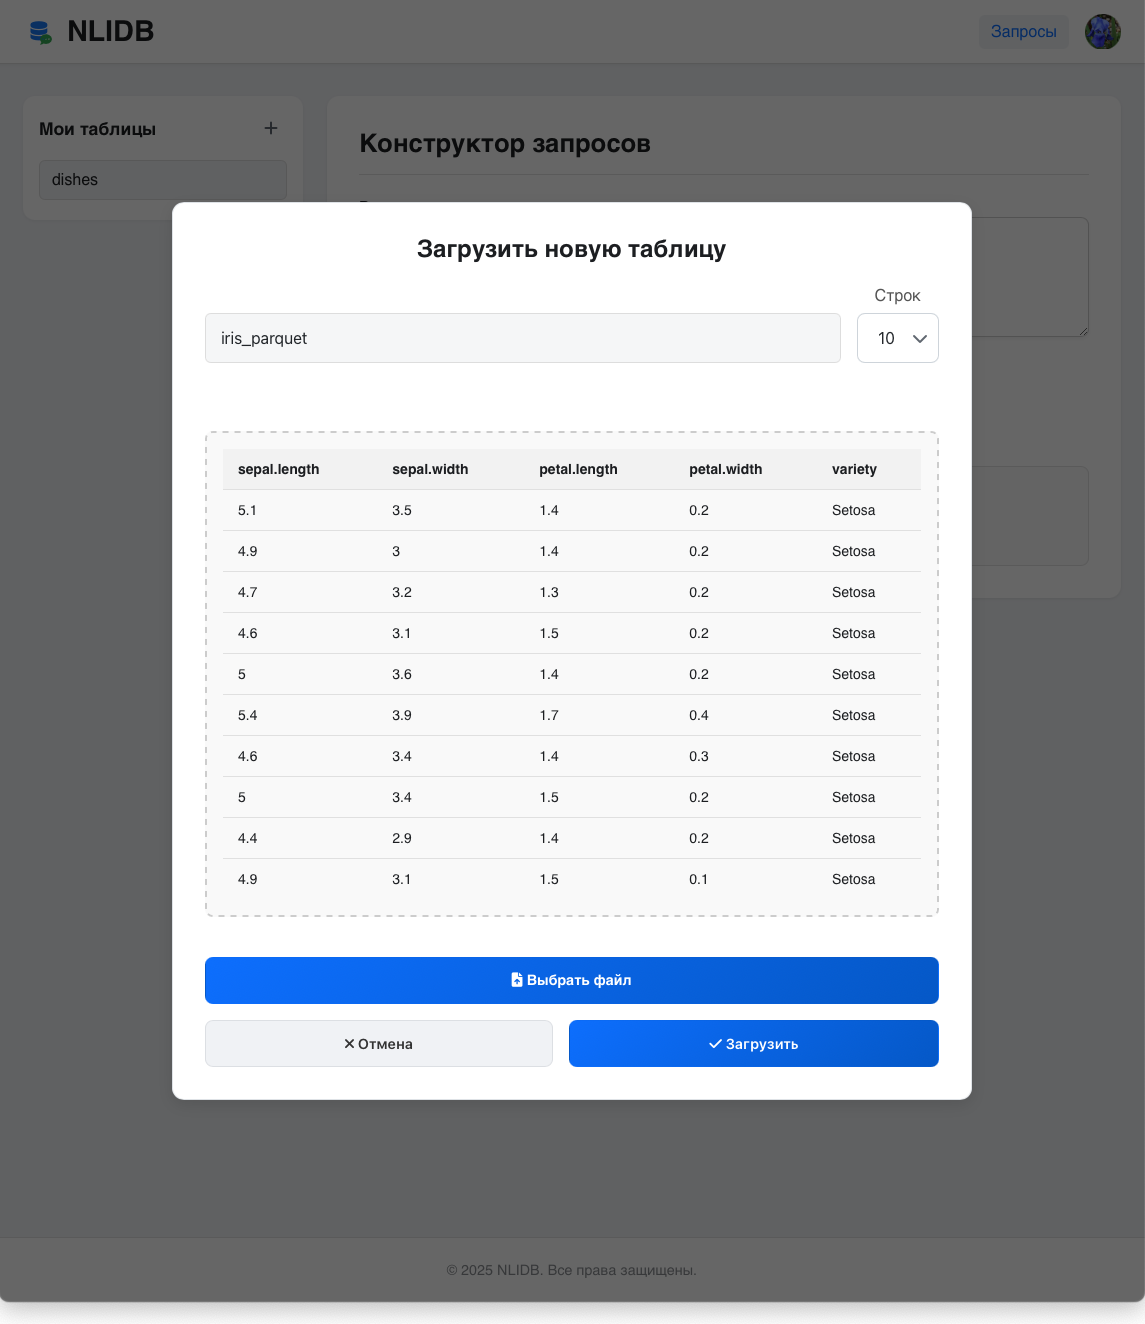
\includegraphics[width=\textwidth]{GUI/table-uploading.png}
      \caption{Модальное окно загрузки и предпросмотра новой таблицы}
      \label{fig:table-uploading}
\end{figure}

Основная часть экрана «Конструктор запросов» содержит большое текстовое поле для ввода запроса на
естественном языке. Ниже расположены кнопки для управления процессом: «Сгенерировать SQL», «Показать
SQL» и «Экспорт в CSV». В области «Результат» отображается таблица с данными, полученными после
выполнения запроса.

\paragraph{Настройки пользователя}. На странице настроек (см.~рис.~\ref{fig:settings}) пользователь
может управлять своим профилем.
Интерфейс разделен на три логических блока:
\begin{compactitem}
      \item \textbf{Смена аватара:} Пользователь может загрузить собственное изображение или удалить
      его, вернувшись к аватару по умолчанию, который генерируется автоматически. Модальное окно для
      смены аватара показано на рис.~\ref{fig:avatar-updating}.
      \item \textbf{Смена имени пользователя:} Поле для изменения псевдонима с мгновенной проверкой
      доступности нового имени.
      \item \textbf{Смена пароля:} Форма для безопасного обновления пароля с подтверждением старого и
      вводом нового пароля с соблюдением требований безопасности.
\end{compactitem}

\begin{figure}[ht]
      \centering
      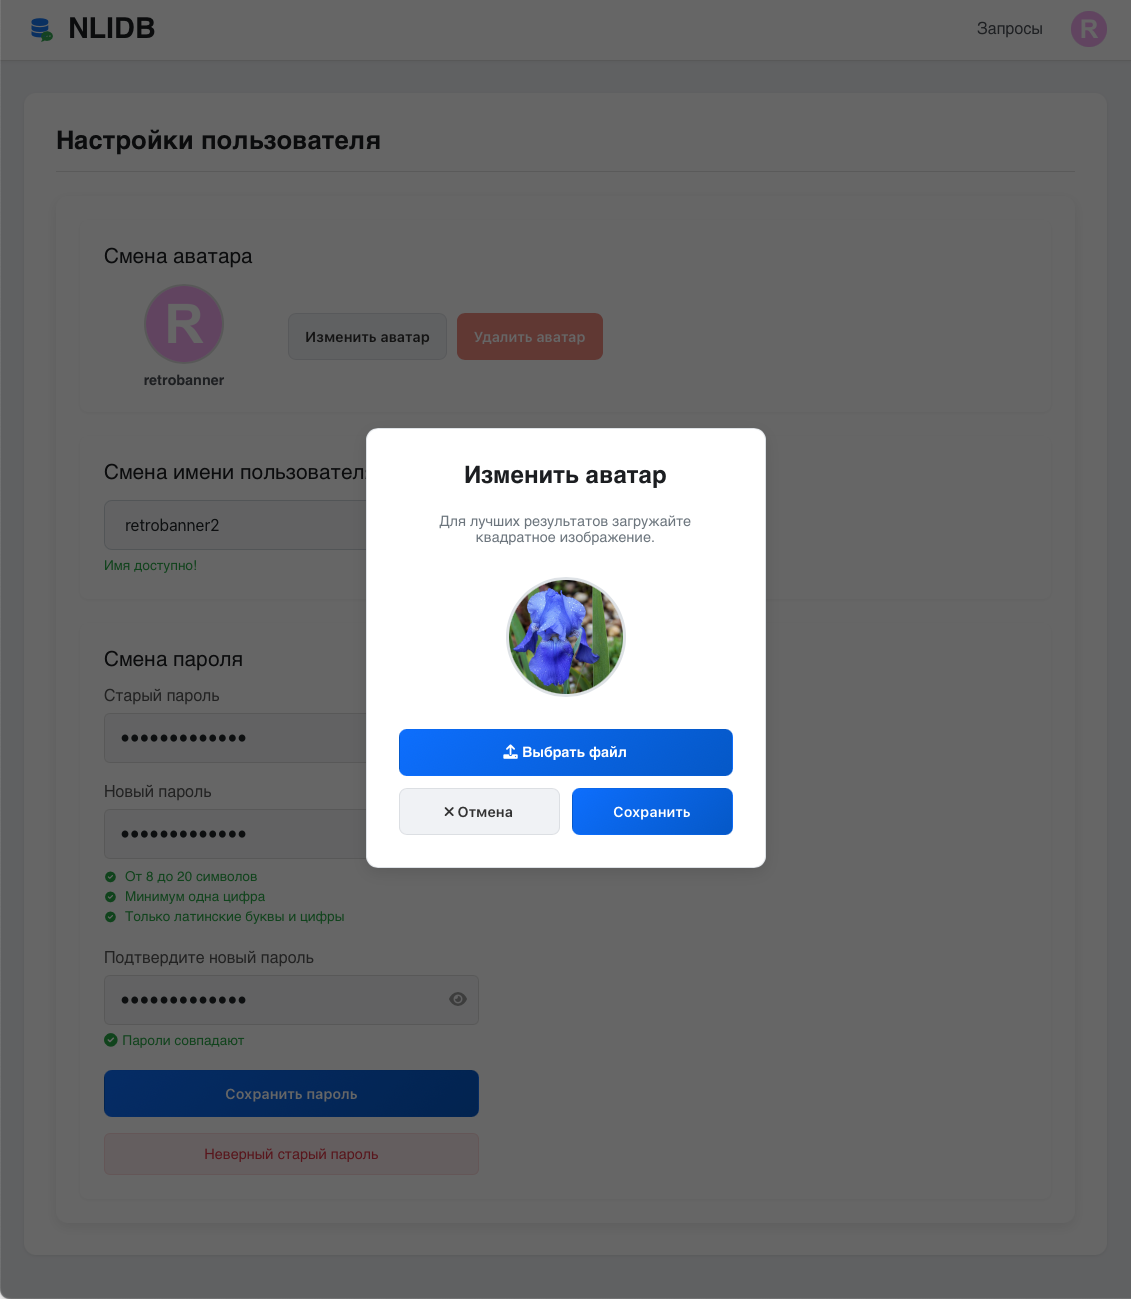
\includegraphics[width=0.8\textwidth]{GUI/avatar-updating.png}
      \caption{Модальное окно смены аватара}
      \label{fig:avatar-updating}
\end{figure}

\begin{figure}[ht]
      \centering
      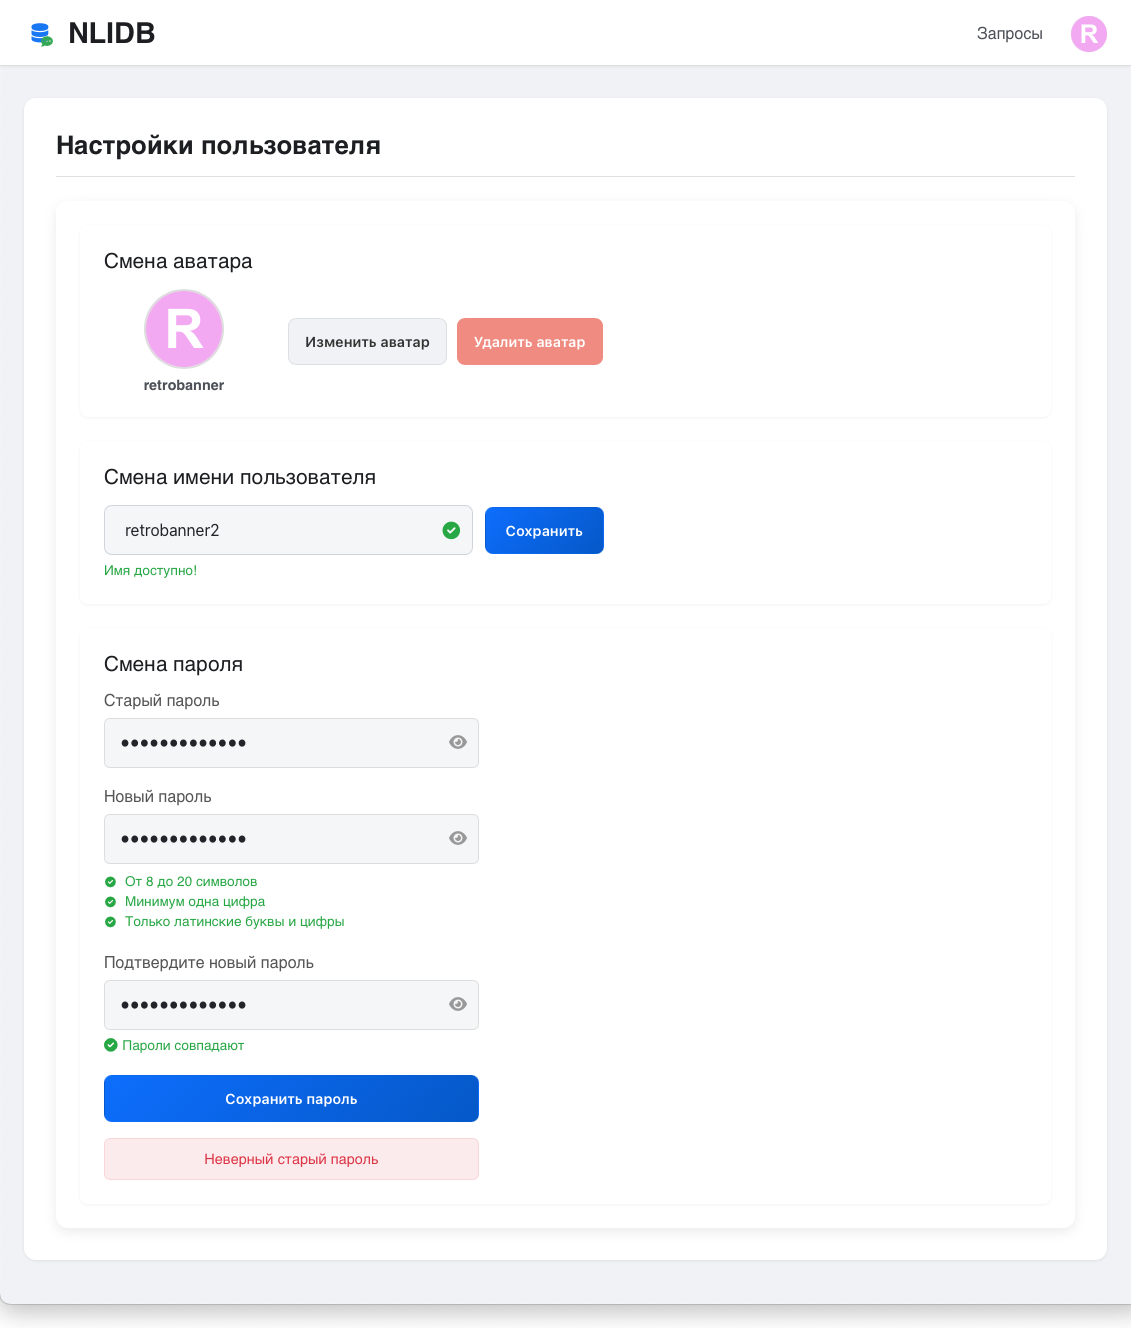
\includegraphics[width=0.8\textwidth]{GUI/settings.png}
      \caption{Страница настроек пользователя}
      \label{fig:settings}
\end{figure}

В целом, спроектированный графический интерфейс является логичным, неперегруженным и полностью
ориентированным на выполнение ключевых задач пользователя, что соответствует целям разработки данного
прототипа.




\section{Тестирование реализованного прототипа веб-сервиса}

Для проверки корректности работы, надежности и соответствия функциональным требованиям, изложенным в
предыдущих разделах, было проведено комплексное модульное тестирование разработанного прототипа.
Тестирование является неотъемлемым этапом жизненного цикла разработки, позволяющим выявить и устранить
потенциальные ошибки на ранней стадии и гарантировать стабильность системы.

\paragraph{Инструменты и среда тестирования}. В качестве основного фреймворка для написания и запуска
тестов был выбран \textbf{pytest}~--- современный и мощный инструмент для тестирования на Python. Для
взаимодействия с API-эндпоинтами приложения использовался \verb|TestClient| из состава фреймворка
FastAPI. Данный подход позволяет отправлять HTTP-запросы напрямую к приложению, не требуя запуска
реального веб-сервера, что значительно ускоряет выполнение тестов и упрощает их настройку.

Для обеспечения полной изоляции тестового окружения все тесты выполнялись на отдельной, временной базе
данных \textbf{SQLite}. Специальная фикстура в \verb|pytest| перед запуском каждого теста создавала
новую, чистую базу данных и удаляла ее после завершения. Это гарантирует, что тесты являются
независимыми друг от друга и результаты одного теста не влияют на последующие.

\paragraph{Структура и организация тестов}. Все автоматизированные тесты расположены в директории
\verb|/tests| и логически сгруппированы в модули, соответствующие структуре основного приложения
(\verb|test_users.py|, \verb|test_tables.py| и т.д.).

Ключевая логика подготовки тестового окружения вынесена в конфигурационный файл
\verb|tests/conftest.py|, где определены основные фикстуры:
\begin{compactitem}
      \item \verb|db|. Управляет жизненным циклом тестовой базы данных, обеспечивая ее создание и
      очистку.
      \item \verb|client|. Предоставляет экземпляр \verb|TestClient| для выполнения запросов от имени
      неаутентифицированного пользователя.
      \item \verb|authorized_client|. Ключевая фикстура для тестирования защищенных эндпоинтов. Она
      инкапсулирует логику создания временного пользователя через API, его последующей аутентификации
      и возвращает клиент с уже установленным токеном авторизации. Это позволяет значительно
      упростить код тестов для защищенных маршрутов.
\end{compactitem}

\paragraph{Тестовое покрытие}. Автоматизированные тесты охватывают все ключевые функциональные модули
разработанного прототипа:
\begin{compactitem}
      \item \textbf{Модуль аутентификации и управления пользователями:} Протестированы сценарии
      регистрации нового пользователя, входа в систему, получения и обновления данных профиля
      (включая смену пароля и аватара). Также покрыты случаи обработки ошибок, такие как попытка
      регистрации с уже существующим именем.
      \item \textbf{Модуль управления таблицами:} Протестированы все CRUD-операции
      (создание, чтение, обновление, удаление) для таблиц данных. Особое внимание уделено проверке
      прав доступа: тесты подтверждают, что пользователь не может получить доступ к таблицам,
      принадлежащим другому пользователю.
      \item \textbf{Внутренние сервисы:} Проведены тесты для отдельных сервисных функций в изоляции, в
      частности, для сервиса \verb|AvatarService|, отвечающего за генерацию аватаров по умолчанию.
\end{compactitem}

\paragraph{Результаты тестирования}. В общей сложности было разработано 47 автоматизированных тестов,
покрывающих описанный выше функционал. \textbf{Все 47 тестов успешно пройдены}, что подтверждается
выводом утилиты \verb|pytest| (см.~прил.~\ref{appendix-C}). В ходе выполнения тестов не было
зафиксировано никаких предупреждений (warnings).

Таким образом, комплексное тестирование подтверждает, что разработанный прототип веб-сервиса
функционирует корректно и в полном соответствии со спроектированной архитектурой и заявленными
функциональными требованиями.